% Options for packages loaded elsewhere
\PassOptionsToPackage{unicode}{hyperref}
\PassOptionsToPackage{hyphens}{url}
\PassOptionsToPackage{dvipsnames,svgnames,x11names}{xcolor}
%
\documentclass[
  number,
  preprint,
  3p,
  twocolumn]{elsarticle}

\usepackage{amsmath,amssymb}
\usepackage{iftex}
\ifPDFTeX
  \usepackage[T1]{fontenc}
  \usepackage[utf8]{inputenc}
  \usepackage{textcomp} % provide euro and other symbols
\else % if luatex or xetex
  \usepackage{unicode-math}
  \defaultfontfeatures{Scale=MatchLowercase}
  \defaultfontfeatures[\rmfamily]{Ligatures=TeX,Scale=1}
\fi
\usepackage{lmodern}
\ifPDFTeX\else  
    % xetex/luatex font selection
\fi
% Use upquote if available, for straight quotes in verbatim environments
\IfFileExists{upquote.sty}{\usepackage{upquote}}{}
\IfFileExists{microtype.sty}{% use microtype if available
  \usepackage[]{microtype}
  \UseMicrotypeSet[protrusion]{basicmath} % disable protrusion for tt fonts
}{}
\makeatletter
\@ifundefined{KOMAClassName}{% if non-KOMA class
  \IfFileExists{parskip.sty}{%
    \usepackage{parskip}
  }{% else
    \setlength{\parindent}{0pt}
    \setlength{\parskip}{6pt plus 2pt minus 1pt}}
}{% if KOMA class
  \KOMAoptions{parskip=half}}
\makeatother
\usepackage{xcolor}
\setlength{\emergencystretch}{3em} % prevent overfull lines
\setcounter{secnumdepth}{3}
% Make \paragraph and \subparagraph free-standing
\ifx\paragraph\undefined\else
  \let\oldparagraph\paragraph
  \renewcommand{\paragraph}[1]{\oldparagraph{#1}\mbox{}}
\fi
\ifx\subparagraph\undefined\else
  \let\oldsubparagraph\subparagraph
  \renewcommand{\subparagraph}[1]{\oldsubparagraph{#1}\mbox{}}
\fi


\providecommand{\tightlist}{%
  \setlength{\itemsep}{0pt}\setlength{\parskip}{0pt}}\usepackage{longtable,booktabs,array}
\usepackage{calc} % for calculating minipage widths
% Correct order of tables after \paragraph or \subparagraph
\usepackage{etoolbox}
\makeatletter
\patchcmd\longtable{\par}{\if@noskipsec\mbox{}\fi\par}{}{}
\makeatother
% Allow footnotes in longtable head/foot
\IfFileExists{footnotehyper.sty}{\usepackage{footnotehyper}}{\usepackage{footnote}}
\makesavenoteenv{longtable}
\usepackage{graphicx}
\makeatletter
\def\maxwidth{\ifdim\Gin@nat@width>\linewidth\linewidth\else\Gin@nat@width\fi}
\def\maxheight{\ifdim\Gin@nat@height>\textheight\textheight\else\Gin@nat@height\fi}
\makeatother
% Scale images if necessary, so that they will not overflow the page
% margins by default, and it is still possible to overwrite the defaults
% using explicit options in \includegraphics[width, height, ...]{}
\setkeys{Gin}{width=\maxwidth,height=\maxheight,keepaspectratio}
% Set default figure placement to htbp
\makeatletter
\def\fps@figure{htbp}
\makeatother

\newpageafter{author}
\makeatletter
\@ifpackageloaded{tcolorbox}{}{\usepackage[skins,breakable]{tcolorbox}}
\@ifpackageloaded{fontawesome5}{}{\usepackage{fontawesome5}}
\definecolor{quarto-callout-color}{HTML}{909090}
\definecolor{quarto-callout-note-color}{HTML}{0758E5}
\definecolor{quarto-callout-important-color}{HTML}{CC1914}
\definecolor{quarto-callout-warning-color}{HTML}{EB9113}
\definecolor{quarto-callout-tip-color}{HTML}{00A047}
\definecolor{quarto-callout-caution-color}{HTML}{FC5300}
\definecolor{quarto-callout-color-frame}{HTML}{acacac}
\definecolor{quarto-callout-note-color-frame}{HTML}{4582ec}
\definecolor{quarto-callout-important-color-frame}{HTML}{d9534f}
\definecolor{quarto-callout-warning-color-frame}{HTML}{f0ad4e}
\definecolor{quarto-callout-tip-color-frame}{HTML}{02b875}
\definecolor{quarto-callout-caution-color-frame}{HTML}{fd7e14}
\makeatother
\makeatletter
\makeatother
\makeatletter
\makeatother
\makeatletter
\@ifpackageloaded{caption}{}{\usepackage{caption}}
\AtBeginDocument{%
\ifdefined\contentsname
  \renewcommand*\contentsname{Table of contents}
\else
  \newcommand\contentsname{Table of contents}
\fi
\ifdefined\listfigurename
  \renewcommand*\listfigurename{List of Figures}
\else
  \newcommand\listfigurename{List of Figures}
\fi
\ifdefined\listtablename
  \renewcommand*\listtablename{List of Tables}
\else
  \newcommand\listtablename{List of Tables}
\fi
\ifdefined\figurename
  \renewcommand*\figurename{Figure}
\else
  \newcommand\figurename{Figure}
\fi
\ifdefined\tablename
  \renewcommand*\tablename{Table}
\else
  \newcommand\tablename{Table}
\fi
}
\@ifpackageloaded{float}{}{\usepackage{float}}
\floatstyle{ruled}
\@ifundefined{c@chapter}{\newfloat{codelisting}{h}{lop}}{\newfloat{codelisting}{h}{lop}[chapter]}
\floatname{codelisting}{Listing}
\newcommand*\listoflistings{\listof{codelisting}{List of Listings}}
\makeatother
\makeatletter
\@ifpackageloaded{caption}{}{\usepackage{caption}}
\@ifpackageloaded{subcaption}{}{\usepackage{subcaption}}
\makeatother
\makeatletter
\@ifpackageloaded{tcolorbox}{}{\usepackage[skins,breakable]{tcolorbox}}
\makeatother
\makeatletter
\@ifundefined{shadecolor}{\definecolor{shadecolor}{rgb}{.97, .97, .97}}
\makeatother
\makeatletter
\makeatother
\makeatletter
\makeatother
\usepackage{float}
\makeatletter
\let\oldlt\longtable
\let\endoldlt\endlongtable
\def\longtable{\@ifnextchar[\longtable@i \longtable@ii}
\def\longtable@i[#1]{\begin{figure}[H]
\onecolumn
\begin{minipage}{0.5\textwidth}
\oldlt[#1]
}
\def\longtable@ii{\begin{figure}[H]
\onecolumn
\begin{minipage}{0.5\textwidth}
\oldlt
}
\def\endlongtable{\endoldlt
\end{minipage}
\twocolumn
\end{figure}}
\makeatother
\ifLuaTeX
  \usepackage{selnolig}  % disable illegal ligatures
\fi
\usepackage[]{natbib}
\bibliographystyle{elsarticle-num}
\IfFileExists{bookmark.sty}{\usepackage{bookmark}}{\usepackage{hyperref}}
\IfFileExists{xurl.sty}{\usepackage{xurl}}{} % add URL line breaks if available
\urlstyle{same} % disable monospaced font for URLs
\hypersetup{
  pdftitle={Longitudinal Analysis Manuscript: Working Draft},
  pdfauthor={Samuel Hawes; Andrew K. Littlefield; Daniel A. Lopez; Kenneth J. Sher; Erin L. Thompson; Raul Gonzalez; Additional Co-authors; Wesley K. Thompson},
  pdfkeywords={ABCD Study, longitudinal analyses, development},
  colorlinks=true,
  linkcolor={blue},
  filecolor={Maroon},
  citecolor={Blue},
  urlcolor={Blue},
  pdfcreator={LaTeX via pandoc}}

\setlength{\parindent}{6pt}
\begin{document}

\begin{frontmatter}
\title{Longitudinal Analysis Manuscript: Working
Draft \\\large{Longitudinal Analysis using data from the ABCD© Study} }
\author[1]{Samuel Hawes%
\corref{cor1}%
}
 \ead{shawes@fiu.edu} 
\author[2]{Andrew K. Littlefield%
%
}
 \ead{andrew.littlefield@ttu.edu} 
\author[3]{Daniel A. Lopez%
%
}
 \ead{Daniel\_Lopez2@URMC.Rochester.edu} 
\author[4]{Kenneth J. Sher%
%
}
 \ead{SherK@missouri.edu} 
\author[5]{Erin L. Thompson%
%
}
 \ead{erthomps@fiu.edu} 
\author[5]{Raul Gonzalez%
%
}
 \ead{gonzara@fiu.edu} 
\author[6]{Additional Co-authors%
%
}
 \ead{xxxxx@fiu.edu} 
\author[7]{Wesley K. Thompson%
%
}
 \ead{wes.stat@gmail.com} 

\affiliation[1]{organization={Florida International University, Center
for Children \& Families},addressline={11200 SW 8th St,
AHC-IV},city={Miami},country={USA},countrysep={,},postcode={33199},postcodesep={}}
\affiliation[2]{organization={Texas Tech University, Psychological
Sciences},city={Lubbock},country={USA},countrysep={,},postcodesep={}}
\affiliation[3]{organization={University of Rochester Medical
Center, Department of Public
Health},city={Rochester},country={USA},countrysep={,},postcodesep={}}
\affiliation[4]{organization={University of Missouri, Psychological
Sciences},city={Columbia},country={USA},countrysep={,},postcodesep={}}
\affiliation[5]{organization={Florida International University, Center
for Children and
Families},city={Miami},country={USA},countrysep={,},postcodesep={}}
\affiliation[6]{organization={xxxxxx University, xxxxxx
Dept},city={xxxx},country={xxxxx},countrysep={,},postcodesep={}}
\affiliation[7]{organization={Laureate Institute for Brain
Research, Center for Population Neuroscience and
Genetics},city={Tulsa},country={USA},countrysep={,},postcodesep={}}

\cortext[cor1]{Corresponding author}








        
\begin{abstract}
The Adolescent Brain Cognitive DevelopmentSM (ABCD) Study presents a
unique opportunity for researchers to investigate developmental
processes in a large, diverse cohort of children and adolescents. Given
the breadth and complexity of the ABCD Study, researchers analyzing its
data are likely to encounter a myriad of methodological and analytic
considerations and concerns. This review provides an examination of key
issues and techniques related to longitudinal data analyses of the ABCD
data. We discuss the value of longitudinal data over cross-sectional
data, focusing on the types of inferences that are possible when one
assesses individuals across multiple time points, including: 1)
characterization of normative variation in developmental trajectories
and the genetic and environmental factors that may lead to deviations
from normative development; 2) assessment of how variation in the
development of one domain may or may not impact development in another;
3) identification of developmental disturbances, snares, and cascade
effects; and 4) relative timing and reciprocal relationships of
within-person changes from different developmental domains. We emphasize
the importance of selecting appropriate methods to address these
research questions, such as accounting for correlation in repeated
measurements and using models for continuous or discrete outcomes as
necessary. By addressing the advantages and potential challenges of
developmental analyses in the ABCD Study, this review seeks to equip
researchers with foundational knowledge and tools to make informed
decisions as they navigate and effectively analyze and interpret the
multi-dimensional longitudinal data currently available.
\end{abstract}





\begin{keyword}
    ABCD Study \sep longitudinal analyses \sep 
    development
\end{keyword}
\end{frontmatter}
    \ifdefined\Shaded\renewenvironment{Shaded}{\begin{tcolorbox}[borderline west={3pt}{0pt}{shadecolor}, breakable, sharp corners, frame hidden, boxrule=0pt, enhanced, interior hidden]}{\end{tcolorbox}}\fi

\hypertarget{introduction}{%
\section{Introduction}\label{introduction}}

\label{sec:headings}
\protect\hypertarget{abcdwebsite}{\href{https://abcdstudy.org/}{The
Adolescent Brain Cognitive Development (ABCD) Study®}} is the largest
long-term investigation of neurodevelopment and child health in the
United States. Conceived and initiated by the National Institutes of
Health (NIH), this landmark prospective longitudinal study aims to
transform our understanding of the genetic and environmental influences
on brain development and their roles in behavioral and health outcomes
in adolescents (Volkow et al.~2018). At its heart, the study is designed
to chart the course of human development across multiple, interacting
domains from late childhood to early adulthood and to identify factors
that lead to both positive and negative outcomes. Central to achieving
these goals is the ABCD Study's® commitment to an open science
framework, intended to facilitate sharing of data and analytical
methods, by espousing practices that increase access, integrity, and
reproducibility of scientific research (e.g., public data releases). In
this sense, the ABCD Study is a collaboration with the larger research
community.

The size and scope of the ABCD Study data allow the research community
to perform a large variety of developmental analyses of both substantive
and methodological interest, presenting a unique opportunity to
significantly advance our understanding of how a multitude of
biopsychosocial processes unfold across critical periods of development.
In this paper we describe models and methods for longitudinal analysis
of ABCD Study data that can address these fundamental scientific aims,
as well as some challenges inherent in a large, longitudinal
observational study of adolescents. We instantiate many of the
longitudinal analyses in worked examples with accompanying R scripts
available at XXXX.

\hypertarget{the-abcd-study-data}{%
\subsection{The ABCD Study Data}\label{the-abcd-study-data}}

The ABCD Study enrolled a large cohort of youth (n=11,880) born between
2006-2008 and aged 9-10 years at baseline, as well as their
parents/guardians. The study sample was recruited from household
populations in defined catchment areas for each of the 21 (originally
22) study sites across the United States. Information regarding funding
agencies, recruitment sites, investigators, and project organization can
be obtained at https://abcdstudy.org/.

The ABCD Study is currently collecting longitudinal data on a rich
variety of outcomes that will enable the construction of complex
statistical models potentially incorporating factors from many domains.
Each new wave of data collection provides another building block for
estimating developmental trajectories and implementing probing
longitudinal analyses that allow researchers to characterize normative
development, to identify variables that presage deviations from
prototypic development, and to assess a range of outcomes associated
with biopsychosocial variables of interest. These data include: 1) a
neurocognitive battery \citep{luciana2018a, thompson2019}; 2) mental and
physical health assessments {[}\citep{barch2018}); 3) measures of
culture and environment \citep{gonzalez2021, zucker2018}; 4) substance
use \citep{lisdahl2021}; 5) biospecimens \citep{uban2018}; 6) structural
and functional brain imaging \citep{casey2018, hagler2019}; 7)
geolocation-based environmental exposure data \citep{fan2021}; 8)
wearables, and mobile technology \citep{bagot2018}; and 9) whole genome
genotyping \citep{loughnan2020}. Many of these measures are collected at
in-person annual visits, with brain imaging collected at baseline and
every other year going forward. A limited number of assessments are
collected in semi-annual telephone interviews between in-person visits.
Data are publicly released on an annual basis, currently through the
NIMH Data Archive.

By necessity, the study's earliest data releases consisted primarily of
cross-sectional (baseline) data; however, the most recent public data
release (Release 5.0) contains data collected across four annual
assessments, including three brain imaging assessments (baseline, year 2
follow-up, and year 4 follow-up visits). Thus, the time is ripe for
implementing a more longitudinal perspective and a focus on estimation
of trajectories (i.e., within-person change over time).

\hypertarget{section}{%
\subsection{}\label{section}}

\begin{tcolorbox}[enhanced jigsaw, coltitle=black, colframe=quarto-callout-note-color-frame, arc=.35mm, title={Organization and Aims}, leftrule=.75mm, toprule=.15mm, titlerule=0mm, breakable, toptitle=1mm, colbacktitle=quarto-callout-note-color!10!white, rightrule=.15mm, colback=white, opacityback=0, bottomtitle=1mm, bottomrule=.15mm, left=2mm, opacitybacktitle=0.6]

• Part I. Longitudinal Research

\begin{itemize}
\tightlist
\item
  Identify fundamental concepts
\end{itemize}

• Part II. Longitudinal Data

\begin{itemize}
\tightlist
\item
  Highlight key challenges
\end{itemize}

• Part III. Longitudinal Analysis

\begin{itemize}
\tightlist
\item
  Learn methods \& analysis to apply
\end{itemize}

• Part IV. Supplemental materials

\begin{itemize}
\tightlist
\item
  Make use of linked open-source resources
\end{itemize}

\end{tcolorbox}

\hypertarget{longitudinal-research}{%
\section{Longitudinal Research}\label{longitudinal-research}}

\label{sec:headings}

\hypertarget{basic-concepts-and-considerations}{%
\subsection{Basic Concepts and
Considerations}\label{basic-concepts-and-considerations}}

There are several important concepts to consider when conducting
longitudinal analyses in a developmental context. These include
different ways of thinking about developmental course, whether certain
periods of development are relatively sensitive or insensitive to
various types of insults or stressors, whether some time periods or
situations inhibit the expression of individual differences due to
extreme environmental pressures, and whether the same behavior
manifested at different times represent the same phenomenon or different
ones. Further, in the case of developmentally focused longitudinal
research, each new measurement occasion not only provides a more
extended portrait of the child's life course but also brings with it
greater methodological opportunities to make use of statistical models
that distinguish within- and between-individual effects and that loosen
constraints that need to be imposed on the furtherance of critical
scientific questions. For example, collecting two or more within-person
observations on the same construct but at different times enables
estimation of within-person rate of change (slopes); more observations
allow for more precise estimates of individual slopes, as well as
characterization of non-linear development. Rate of change or other
aspects of trajectory shapes may be more informative than the simple
snapshots of level differences that cross-sectional data are limited to.
Appreciation of these and other issues can help to guide the analysis
and interpretation of data and aid translation to clinical and public
health applications.

\hypertarget{vulnerable-periods.}{%
\subsubsection{Vulnerable periods.}\label{vulnerable-periods.}}

Adolescent development progresses normaly from less mature to more
mature levels of functioning. However, unique epochs and experiences can
alter the course of this idealized form of development. Consider
research that shows cannabis use during adolescence is associated with
later psychosis to a greater degree than cannabis use initiated later in
development \citep{arseneault2002, bechtold2016, hasan2020, semple2005};
or, similarly, experimental research on rodents that shows rodent brains
to be especially sensitive to the neurotoxic effects of alcohol on brain
structure and learning early in development (corresponding to early
adolescence in humans) \citep{spear2016, crews2000, ji2018}. For
example, longitudinal data from the National Consortium on Alcohol in
Adolescence (NCANDA) show that binge drinking is associated more
strongly with decrements in gray matter volume early in adolescence
compared to later \citep{infante2022}. These examples highlight the
importance of considering the role of vulnerable periods -- e.g.,
temporal windows of rapid brain development or remodeling during which
the effects of environmental stimuli (e.g.~alcohol exposure) on the
developing brain may be particularly pronounced-- when trying to
establish an accurate understanding of the association between exposures
and outcomes.

\hypertarget{developmental-disturbances.}{%
\subsubsection{Developmental
disturbances.}\label{developmental-disturbances.}}

Whereas vulnerable periods heighten neurobiological susceptibility to
environmental influences, at other times, environmental presses will
tend to suppress stability and disrupt the orderly stochastic process of
normative development \citep[e.g.,][]{schulenberg2019}. This situation
reflects a developmental disturbance in that the normal course of
development is ``altered'' by some time-limited process. In such cases,
we might find that prediction of behavior in the period of the
disturbance is reduced and/or, similarly, the behavior exhibited during
the disturbance might have less predictive power with respect to distal
outcomes compared to the behavior exhibited before and following the
disrupted period. That is, once the environmental pressures are removed
(or the individual is removed from the environment), patterns of
individual differences (and autoregressive effects) recover to levels
similar to those prior to entering the environment. For example, in
\citep{infante2022}, recent binge drinking appears to be most predictive
of gray matter volume trajectories, as opposed to prior binge drinking
or cumulative number of binge drinks, suggesting the potential for
recovery of gray matter trajectories to prior levels of growth if binge
drinking subsides.

\hypertarget{developmental-snares-and-cascade-effects.}{%
\subsubsection{Developmental snares and cascade
effects.}\label{developmental-snares-and-cascade-effects.}}

Normative development can also be upended by experiences (e.g., drug
use) that, through various mechanisms, disrupt the normal flow of
development wherein each stage establishes a platform for the next. For
instance, substance use could lead to association with other
substance-using or rule-breaking peers, precluding opportunities for
learning various adaptive skills and prosocial behaviors, in effect
creating a ``snare'' that delays psychosocial development, such as
maturing out of adolescent antisocial behavior \citep{moffitt2015}.
Relatedly, the consequences of these types of events can cascade (e.g.,
school dropout, involvement in the criminal justice system) so that the
effects of the snare are amplified
\citep[e.g.,][]{masten2005, rogosch2010}. Although conceptually distinct
from vulnerable periods, both types of developmental considerations
highlight the importance of viewing behavior in the context of
development and the importance of attempting to determine how various
developmental pathways unfold. Longitudinal data are crucial in this
context to assess individual levels of development prior to and
following onset of experiences or other environmental factors; e.g., the
ABCD Study collected data starting at ages 9-10 and hence before the
onset of drug use for the vast majority of participants.

\hypertarget{longitudinal-data}{%
\section{Longitudinal Data}\label{longitudinal-data}}

\label{sec:headings}

\hypertarget{interpretation-issues-pitfalls-assumption}{%
\subsection{Interpretation / Issues / Pitfalls \&
Assumption}\label{interpretation-issues-pitfalls-assumption}}

The hallmark characteristic of longitudinal data analysis is the
administration of repeated measurements of the same constructs on
assessment targets (e.g., individuals, families) across time. The
primary rationale for collecting longitudinal data is to assess
within-person change over time, allowing researchers to estimate
individual developmental trajectories and the genetic and/or
environmental factors that may impact these. Generally speaking,
administering repeated measurements more frequently or over longer time
spans enables researchers to ask more nuanced questions and to make
stronger inferences.

\hypertarget{two-time-points-versus-three-or-more.}{%
\subsubsection{Two Time Points versus Three or
More.}\label{two-time-points-versus-three-or-more.}}

Although the clear leap from cross-sectional to the realm of
longitudinal data involves going from one assessment to two or more
assessments, there are also notable distinctions in designs based on
two-assessment points versus three or more measurement occasions. Just
as cross-sectional data can be informative in some situations, two waves
of data can be beneficial in contexts such as when experimental
manipulation is involved (e.g., pre/post tests), or if the central goal
is prediction (e.g., trying to predict scores on Variable A at time T as
a function of prior scores on Variable A and Variable B at time T-1). At
the same time, data based on two assessments are inherently limited on
multiple fronts. As \citep{rogosa1982} noted over forty years ago, ``Two
waves of data are better than one, but maybe not much better'' (p XX).

These sentiments are reflected in more contemporary recommendations
regarding best-practice guidelines for prospective data, which
increasingly emphasize the benefits of additional measurement occasions
for trajectory estimation, model identification and accurate parameter
estimation. It is also consistent with research recommending that
developmental studies include three or more assessment points, given it
is impossible for data based on two-time points to determine the shape
of development, since linear change is the only estimable form given two
assessments \citep[see][]{duncan2009}. Research designs that include
three (but preferably more) time points allow for non-linear trajectory
estimation and increasingly nuanced analyses that more adequately tease
apart sources of variation and covariation among the repeated
assessments {[}\citep{king2018})-- a key aspect of developmental
research.

To illustrate, developmental theories are useful for understanding
patterns of within-individual change over time (discussed in further
detail, below); however, two data points provide meager information on
change at the person level. This point is further underscored in a
recent review of statistical models commonly touted as distinguishing
within-individual vs between-individual sources of variance in which the
study authors concluded ``\ldots{} researchers are limited when
attempting to differentiate these sources of variation in psychological
phenomenon when using two waves of data'' and perhaps more concerning,
``\ldots the models discussed here do not offer a feasible way to
overcome these inherent limitations'' \citep{littlefield2021}.

It is important to note, however, that despite the current focus on
two-wave designs versus three or more assessment waves, garnering three
assessment points is not a panacea for longitudinal modeling. Indeed,
several contemporary longitudinal models designed to isolate
within-individual variability {[}e.g., the Latent Curve Model with
Structured Residuals; \citep{curran2014}{]} require at least four
assessments to parameterize fully and, more generally, increasingly
accurate parameter estimates are obtained as more assessment occasions
are used \citep{duncan2009}.

\hypertarget{types-of-stability-and-change}{%
\subsubsection{Types of stability and
change}\label{types-of-stability-and-change}}

If one were to try to sum up what developmental trajectories in a living
organism are exactly, one could plausibly argue they are the patterns of
stability and change in its phenotypes as the organism traverses the
life course. Mathematically, this could be expressed as f(t), a possibly
multivariate function of time t typically taking values in the real
numbers for continuous phenotypes or the integers for discrete
phenotypes. There are a few different ways to think about patterns of
stability and change (see Figure 1). Consider measuring the height of
all youth in a 6th-grade class, once in the fall at the beginning of the
school year and once again in the spring at the end of the school year.
A common first step may be to compare the class's average height values
obtained at these two different measurement occasions. This comparison
of the average scores for the same group of individuals at multiple time
points is referred to as ``mean-level'' stability, as it provides
information about continuity and change over time for an outcome of
interest, aggregated across members of a group.

In contrast, ``between-individual'' stability and change could be
assessed, e.g., by calculating the Spearman correlation between the
values obtained at different time points (e.g., `height in the fall'
with `height in the spring'). This analysis focuses on the degree to
which individuals retain their relative placement in a group across
time. Consider someone who is the shortest person in their class in 6th
grade may grow considerably over the school year (i.e., exhibit mean
level change), but remain the shortest person among their classmates.
That is, the individual is manifesting a type of rank-order stability.

Both types of stability and change are important. Mean-level change in
certain traits might help to explain why, in general, individuals tend
to be particularly vulnerable to the effects of environmental factors at
some ages more than others; rank-order stability might help to quantify
the extent to which certain characteristics of the individual are more
trait-like. For example, in some areas of development, there is
considerable mean-level change that occurs over time {[}e.g., changes in
Big 5 personality traits; \citep{bleidorn2022}{]}, but relatively high
rank-order stability, at least over relatively shorter measurement
intervals \citep{bleidorn2022, roberts2000, roberts2006}. Despite the
useful information afforded by examining mean-level and rank-order
stability, these approaches are limited in that they provide little
information about the patterns of within-individual change (i.e.,
trajectories) and, in turn, can result in fundamental misinterpretations
about substantial or meaningful changes in an outcome of interest
\citep{curran2011}.

\begin{figure}

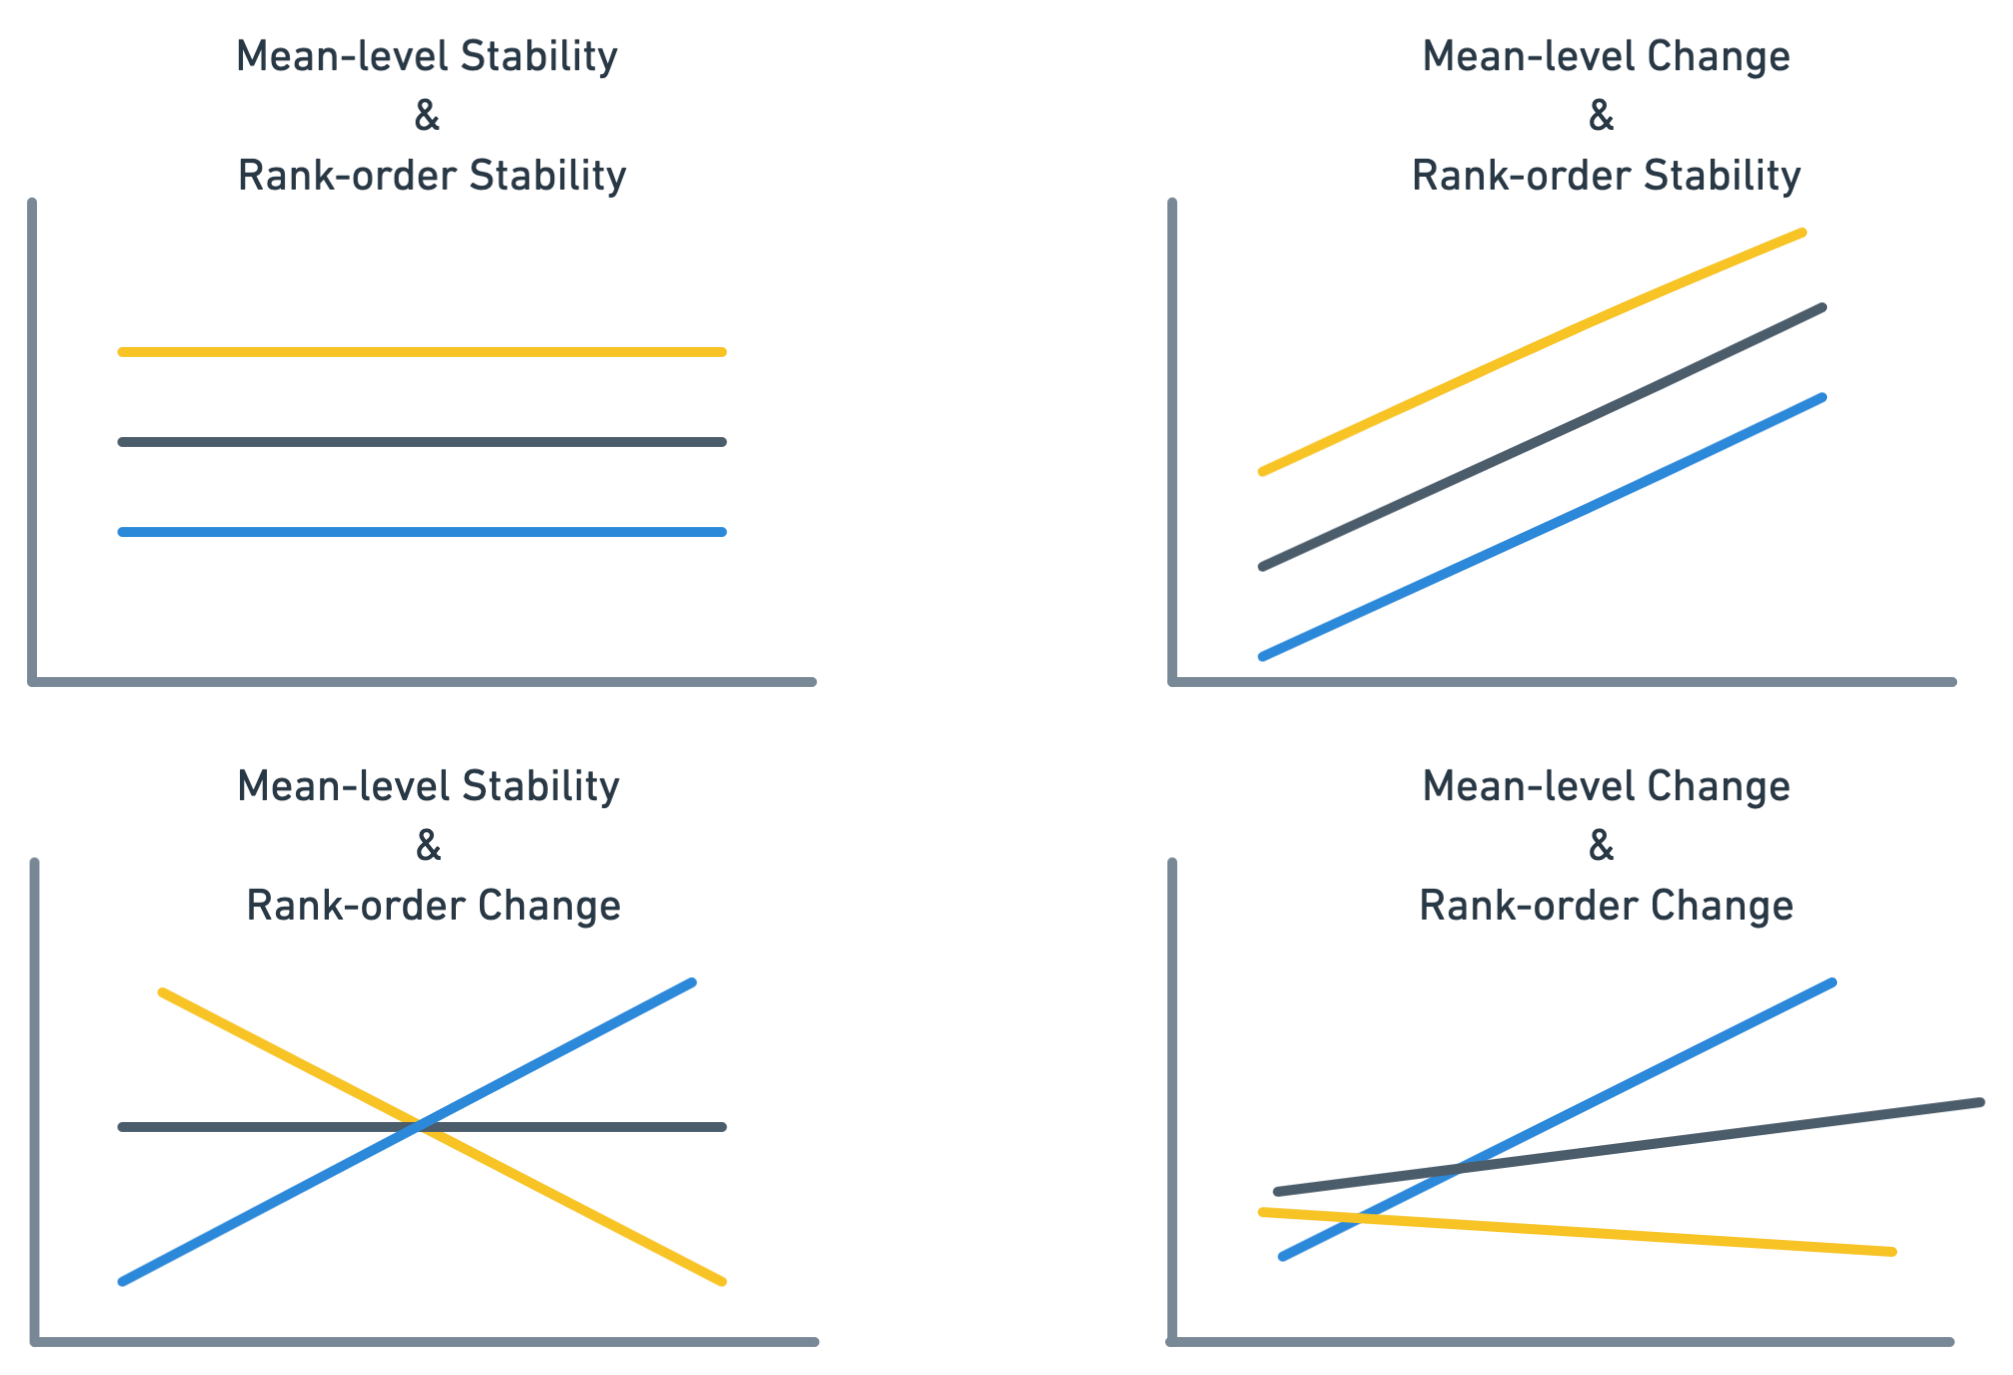
\includegraphics[width=3.125in,height=3.125in]{./figures/StabilityChange.png} \hfill{}

\caption{\label{fig-StablityChange}Types of Stability and Change}

\end{figure}

There is growing recognition that statistical models commonly applied to
longitudinal data often fail to align with the developmental theory they
are being used to assess
\citep[e.g.,][]{curran2011, hoffman2015, littlefield2021}. Specifically,
developmental studies typically involve the use of prospective data to
inform theories that are concerned with clear within-person (i.e.,
intraindividual) processes (e.g., how phenotypes change or remain stable
within individuals over time) \citep[e.g.,][]{curran2011}. Despite this,
methods generally unsuited for disaggregating between- and within-person
effects (e.g., cross-lagged panel models {[}CLPM{]}) remain common
within various extant literatures. Fortunately, there exists a range of
models that have been proposed to tease apart between- and within-person
sources of variance across time
\citep[see][]{littlefield2021, orth2021}. Most of these contemporary
alternatives incorporate time-specific latent variables to capture
between-person sources of variance and model within-person deviations
around an individual's mean (or trait) level across time such as the
random-intercept crosslagged panel model \citep[e.g.,
RI-CLPM,][]{hamaker2015} and the latent curve model with structured
residuals \citep[e.g., LCM-SR,][]{curran2014}. It is important to note
however that these models require multiple assessments waves (e.g., four
or more to fully specify the LCM-SR), additional expertise to overcome
issues with model convergence, and appreciation of modeling assumptions
when attempting to adjudicate among potential models in each research
context \citep[see][for further discussion]{littlefield2021}.

\hypertarget{model-assumptions}{%
\subsubsection{Model assumptions}\label{model-assumptions}}

Many statistical models assume certain characteristics about the data to
which they are being applied. Common assumptions of parametric
statistical models (e.g., linear mixed-effects models) include
normality, linearity, and equality of variances. These assumptions must
be carefully considered before conducting analysis so that valid
inferences can be made from the data, as violation of a model's
assumptions can substantively invalidate the interpretation of results.
For example, longitudinal data can exhibit heterogeneous variability
(i.e., the variance of the response changes over the duration of the
study) that may need to be accounted for within a model. Similarly,
longitudinal measurement invariance can help to establish whether or not
a construct is measured consistently over time
\citep{liu2017, van2015, willoughby2012}, providing researchers with
greater confidence that any change over time identified for a construct
is attributable to individual change rather than a measurement artifact.

\hypertarget{distinguishing-developmental-change-from-experience-effects}{%
\subsubsection{Distinguishing developmental change from experience
effects}\label{distinguishing-developmental-change-from-experience-effects}}

One can often observe systematic changes over time in a variable of
interest and assume this change is attributable to development. To this
point, cognitive abilities (e.g, verbal ability, problem-solving)
normatively grow earlier in development and often decline in late life
(e.g., memory, speed of processing). However, the observed patterns of
growth and decline often differ between cross-sectional vs.~longitudinal
effects \citep{salthouse2014} where subjects gain increasing experience
with the assessment during each successive measurement occasion. Such
experience effects on cognitive functioning have been demonstrated in
adolescent longitudinal samples similar to ABCD {[}\citep{sullivan2017})
and highlight the need to consider these effects and address them
analytically. In the case of performance-based measures {[}e.g., matrix
reasoning related to neurocognitive functioning; see
\citep{salthouse2014}{]}, this can be due to ``learning'' the task from
previous test administrations (e.g., someone taking the test a second
time performs better than they did the first time simply as a function
of having taken it before). Even in the case of non-performance-based
measures (e.g., levels of depression), where one cannot easily make the
argument that one has acquired some task-specific skill through
learning, it has been observed that respondents tend to endorse lower
levels on subsequent assessments \citep[e.g.,][]{beck1961, french2010}
and this phenomenon has been well documented in research on structured
diagnostic interviews \citep{robins1985}. While it is typically assumed
that individuals are rescinding or telling us less information on
follow-up interviews, there is reason to suspect that in some cases the
initial assessment may be artifically elevated {[}see
\citep{shrout2018}). Some designs (specifically, accelerated
longitudinal designs) are especially well suited for discovering these
effects and modeling them. While ABCD was not designed as an accelerated
longitudinal design, the variability in age at the time of baseline
recruitment (9 years, 0 months to 10 years, 11 months) allows some
measures, collected every year, to be conceptualized as an accelerated
longitudinal design\ldots albeit to a modest extent. It is possible that
in later waves, analyses will allow for disaggregating the confounded
effects of age and the number of prior assessments. However, ABCD is
fundamentally a single-cohort, longitudinal design, wherein the number
of prior assessments and age may be confounded. As such, the possible
influence of experience effects needs to be kept in mind.

\hypertarget{covariance-structures}{%
\subsubsection{Covariance Structures}\label{covariance-structures}}

A central issue for repeated measurements on an individual is how to
account for the correlated nature of the data. Traditional techniques,
such as a standard regression or ANOVA model, assume residuals are
independent and thus are inappropriate for designs that assess the same
individuals across time. That is, given that residuals are no longer
independent, the standard errors from the models are biased and can
produce misleading inferential results. Although there are formal tests
of independence for time series data (e.g., the Durbin-Watson statistic
\citep{durbin1950}, independence is more commonly, independence is
assumed to be violated in study designs with repeated assessments.
Therefore, an initial question to be addressed by a researcher analyzing
prospective data is how to best model the covariance structure of said
data.

Statistical models for longitudinal data include two main components to
account for assumptions that are commonly violated when working with
repeated measures data: a model for the covariance among repeated
measures (involving the covariance among pairs of repeated outcomes on
an individual), coupled with a model for the mean response and its
dependence on covariates (e.g., sex at birth). There exists a range of
methods to model covariance structures, each with its own set of
tradeoffs between model fit and parsimony and which may be more or less
appropriate for each specific application {[}e.g., see
\citep{kincaid2005}).

One alternative structure that attempts to handle the reality that
correlations between repeated assessments tend to diminish across time
is the autoregressive design. As the name implies, the structure assumes
a subsequent measurement occasion (e.g., assessment at Wave 2) is
regressed onto (that is, is predicted by) a prior measurement occasion
(e.g., assessment at Wave 1). The most common type of autoregressive
design is the AR(1), where assessments at time T + 1 are regressed on
assessments at Time T. Identical to compound symmetry, this model
assumes the variances are homogenous across time. Diverting from
compound symmetry, this model assumes the correlations between repeated
assessments decline exponentially across measurement occasions rather
than remaining constant. That is, we can think of the underlying process
as a stochastic one that wears itself out over time. For example, per
the AR(1) structure, if the correlation between Time 1 and Time 2 data
is thought to be .5, then the correlation between Time 1 and Time 3 data
would be assumed to be .5 × .5 = .25, and the correlation between Time 1
and Time 4 data would be assumed to be .5 × .5 × .5 = .125. As with
compound symmetry, the basic AR(1) model is parsimonious in that it only
requires two parameters (the variance of the assessments and the
autoregressive coefficient). Notably, the assumption of constant
autoregressive relations between assessments is often relaxed in
commonly employed designs that use autoregressive modeling (e.g.,
cross-lagged panel models {[}CLPM{]}). These designs still typically
assume an AR(1) process (e.g., it is sufficient to regress the Time 3
assessment onto the Time 2 assessment and is not necessary to also
regress the Time 3 assessment onto the Time 1 assessment, which would
result in an AR(2) process). However, the magnitude of these relations
is often allowed to differ across different AR(1) pairs of assessment
(e.g., the relation between Time 1 and Time 2 can be different from the
relation between Time 2 and Time 3). These more commonly employed models
also often relax the assumption of equal variances of the repeated
assessments. Although the AR(1) structure may involve a more realistic
set of assumptions compared to compound symmetry, in that the AR(1)
model allows for diminishing correlations across time, the basic AR(1)
model, as well as autoregressive models more generally, can also suffer
from several limitations in contexts that are common in prospective
designs. In particular, recent work demonstrates that if a construct
being assessed prospectively across time is trait-like in nature, then a
simple AR(1) process fail to adequately account for this trait-like
structure, with the downstream consequence that estimates derived from
models based on AR structures (such as the CLPM) can be misleading and
fail to adequately demarcate between- vs.~within-person sources of
variance \citep{hamaker2015}. Finally, it is also worth noting that in
many longitudinal contexts, the time intervals between assessments are
not equidistant and researchers need to consider carefully how to
appropriately model time in their model and what this model implies.

\hypertarget{continuous-and-discrete-outcomes}{%
\subsubsection{Continuous and Discrete
Outcomes}\label{continuous-and-discrete-outcomes}}

Identification of valid and efficient statistical models requires an
understanding of the type of data being analyzed. For example, repeated
assessments can be based on continuous or discrete measures. Examples of
discrete measures include repeated assessments of binary variables
(e.g., past 12-month alcohol use disorder status measured across ten
years), ordinal variables (e.g., a single item measuring the level of
agreement to a statement on a three-point scale including the categories
of ``disagree'', ``neutral'', and ``agree'' in an ecological momentary
assessment study that involves multiple daily assessments), and count
variables (e.g., number of cigarettes smoked per day across a daily
diary study). In many ways, the distributional assumptions of indicators
used in longitudinal designs mirror the decision points and
considerations when delineating across different types of discrete
outcome variables, a topic that spans entire textbooks \citep[e.g.,
see][]{lenz2016}. For example, the Mplus manual \citep{muthen2017}
includes examples of a) censored and censored-inflated models, b) linear
growth models for binary or ordinal variables, c) linear growth models
for a count outcome assuming a Poisson model, and d) linear growth
models for a count outcome assuming a zero-inflated Poisson model.
Beyond these highlighted examples, other distributions (e.g., negative
binomial) can be assumed for the indicators when modeling longitudinal
data \citep{ren2022}. These models can account for issues that can occur
when working with discrete outcomes, including overdispersion {[}when
the variance is higher than would be expected based on a given
distribution; see \citep{lenz2016}{]}. Given the sheer breadth of issues
relevant to determining better models for discrete outcomes, it is not
uncommon for texts on longitudinal data analysis to only cover models
and approaches that assume continuous variables
\citep[e.g.,][]{little2013}. However, some textbooks on categorical data
analysis provide more detailed coverage of the myriad issues and
modeling choices to consider when working with discrete outcomes
{[}e.g., \citep{lenz2016}, Chapter 11 for matched pair/two-assessment
designs; Chapter 12 for marginal and transitional models for repeated
designs, such as generalized estimating equations, and Chapter 13 for
random effects models for discrete outcomes{]}.

\hypertarget{missing-dataattrition}{%
\subsubsection{Missing Data/Attrition}\label{missing-dataattrition}}

As recently reviewed by \citep{littlefield2022}, investigators of
prospective data are confronted by the certain prospect of study
attrition (i.e., participants may not provide data at a given wave of
assessment or may drop out of the study altogether) and thus approaches
are needed to confront the issue of missing data. Three types of
missingness are typically considered in the literature
\citep[see][]{little1989}, namely: a) missing completely at random
(MCAR), b) missing at random (MAR), and c) missing not at random (MNAR).
Data that are MCAR means that the missing data are a simple random
sample of all data in a given dataset. MAR means missing at random
conditional on the observed covariates \citep[see][]{graham2009}. That
is, MAR implies missing data are a random sample (i.e., does not hinge
on some unmeasured variables) within strata of the measured covariates
in a dataset (e.g., biological sex). Data that are MNAR are missing as a
function of unobserved variables and may bias assocaitions even after
conditioning on the observed covariates. \citep{graham2009} provides an
excellent and easy-to-digest overview of further details involving
missing data considerations.

Multiple approaches have been posited to handle missing data. Before the
advent of more contemporary approaches, common methods included several
ad hoc procedures. These include eliminating the data of participants
with missing data (e.g., listwise or pairwise deletion) or using mean
imputation (i.e., replacing the missing value with the mean score of the
sample that did participate). However, these methods are not recommended
because they can contribute to biased parameter estimates and research
conclusions \citep[see][]{graham2009}. Another common approach to
imputing missing data is termed ``last observation carried forward''
(LOCF). LOCF replaces a participant's missing values after dropout with
the last available measurement \citep{molnar2008}. This approach assumes
stability (i.e., a given participant's score is not anticipated to
systematically increase or decline after study dropout) and that the
data are MCAR. However, as described by \citep{molnar2008}, it is common
for treatment groups to show higher attrition compared to control groups
in studies of dementia drugs. Given that dementia worsens over time,
using LOCF biases the results in favor of the treatment group
\citep[see][for more details]{molnar2008}.

More modern approaches, such as full information maximum likelihood,
propensity weighting, auxiliary variables and multiple imputation avoid
some of the biases of older approaches
\citep[see][]{enders2010, graham2009}. \citep{graham2009} noted several
``myths'' regarding missing data. For example, Graham notes many assume
the data must be minimally MAR to permit estimating procedures (such as
maximum likelihood or multiple imputation) compared to other, more
traditional approaches (e.g., using only complete case data). Violations
of MAR impact both traditional and more modern data estimation
procedures, though as noted by Graham, violations of MAR tend to have a
greater effect on older methods. Graham thus suggests that imputing
missing data is a better approach compared to the older procedures in
most circumstances, regardless of the model of missingness {[}i.e.,
MCAR, MAR, MNAR; see \citep{graham2009}{]}.

Attrition from a longitudinal panel study such as ABCD is inevitable and
represents a potential threat to the validity of longitudinal analyses
and cross-sectional analyses conducted at later time points, especially
since attrition can only be expected to grow over time. The ABCD
Retention Workgroup (RW) employs a data-driven approach to examine,
track, and intervene in these issues and while preliminary findings show
participant race and parent education level to be associated with late
and missing visits, although to date, attrition in ABCD has been minimal
\citep{ewing2022}. Ideally, one tries to minimize attrition through good
retention practices from the outset via strategies designed to maintain
engagement in the project \citep{cotter2005, hill2016, watson2018}.
However, even the best-executed studies need to anticipate growing
attrition over the length of the study and implement analytic strategies
designed to provide the most valid inferences. Perhaps the most key
concern when dealing with data that is missing due to attrition is
determining the degree of bias in retained variables that is a
consequence of attrition. Such bias can attenuate generalizability,
particularly if the pattern of missingness is not random (e.g., certain
subsets of the population are more likely to drop out/not attend a
visit). Assuming that the data are not missing completely at random,
attention to the nature of the missingness and employing techniques
designed to mitigate attrition-related biases need to be considered in
all longitudinal analyses.

\hypertarget{quantifying-effect-sizes-longitudinally}{%
\subsubsection{Quantifying effect sizes
longitudinally}\label{quantifying-effect-sizes-longitudinally}}

Given longitudinal data involve different sources of variance,
quantifying effect sizes longitudinally is a more difficult task
compared to deriving such estimates from cross-sectional data. Effect
size can be defined as, ``a population parameter (estimated in a sample)
encapsulating the practical or clinical importance of a phenomenon under
study.'' \citep{kraemer2014}. Common effect size metrics include r
(i.e., the standardized covariance, or correlation, between two
variables) and Cohen's d {[}i.e., the standardized difference between
two means; \citep{cohen1988}{]}. Adjustments to common effect size
calculations, such as Cohen's d, are required even when only two time
points are considered \citep[e.g., see][]{morris2002}. \citep{wang2019}
note there are multiple approaches to obtaining standardized
within-person effects, and that commonly suggested approaches (e.g.,
global standardization) can be problematic \citep[see][for more
details]{wang2019}. Thus, obtaining effect size metrics based on
standardized estimates that are relatively simple in cross-sectional
data (such as r) becomes more complex in the context of prospective
data. \citep{feingold2009} noted that equations for effects sizes used
in studies involving growth modeling analysis (e.g., latent growth curve
modeling) were not mathematically equivalent, and the effect sizes were
not in the same metric as effect sizes from traditional analysis
\citep[see][for more details]{feingold2009}. Given this issue, there
have been various proposals for adjusting effect size measures in
repeated assessments. \citep{feingold2019} reviews the approach for
effect size metrics for analyses based on growth modeling, including
when considering linear and non-linear (i.e., quadratic) growth factors.
\citep{morris2002} review various equations for effect size calculations
relevant to combining estimates in meta-analysis with repeated measures
and independent-groups designs. Other approaches to quantifying effect
sizes longitudinally may be based on standardized estimates from models
that more optimally disentangle between- and within-person sources of
variance (as reviewed above). As an example, within a random-intercept
cross-lagged panel model (RI-CLPM) framework, standardized estimates
between random intercepts (i.e., the correlation between two random
intercepts for two different constructs assessed repeatedly) could be
used to index the between-person relation, whereas standardized
estimates among the structured residuals could be used as informing the
effect sizes of within-person relations.

\hypertarget{longitudinal-data-structures}{%
\subsubsection{Longitudinal Data
Structures}\label{longitudinal-data-structures}}

An ideal longitudinal study integrates (a) a well-articulated
theoretical model, (b) an appropriate longitudinal data structure, and
(c) a statistical model that is an operationalization of the theoretical
model \citep{collins2006}. To accommodate various research questions and
contexts, different types of longitudinal data and data structures have
emerged (see Figure x). An understanding of these data structures is
helpful, as they can warrant different types of longtiudinal data
analysis. Given that identifying a starting point for making comparisons
is somewhat arbitrary, \citep{bauer2019} provide a nice on-ramp in first
distinguishing between the use of ``time-to-event'' and ``repeated
measures'' data. Although both model time, the former is concerned with
whether and when an event occurs, whereas the later is focused on growth
and change \citep{bauer2019}. Time-to-event structures measure time from
a well-defined origin point up to the occurrence of an event of
interest. This data structure is most often analyzed using survival
analysis methods (e.g., hazard rate models, event history analysis,
failure-time models) and the time-to-event data can be based on a single
assessment or include multiple recurrent or competing events. While much
has been written about ``time-to-event'' data (see xxx; xxx; xxxx),
including several recent xxxx (see), our emphasis will be given to the
modeling of ``repeated measures'' data.

\begin{figure}

{\centering 

\href{https://centerstat.org/resources/}{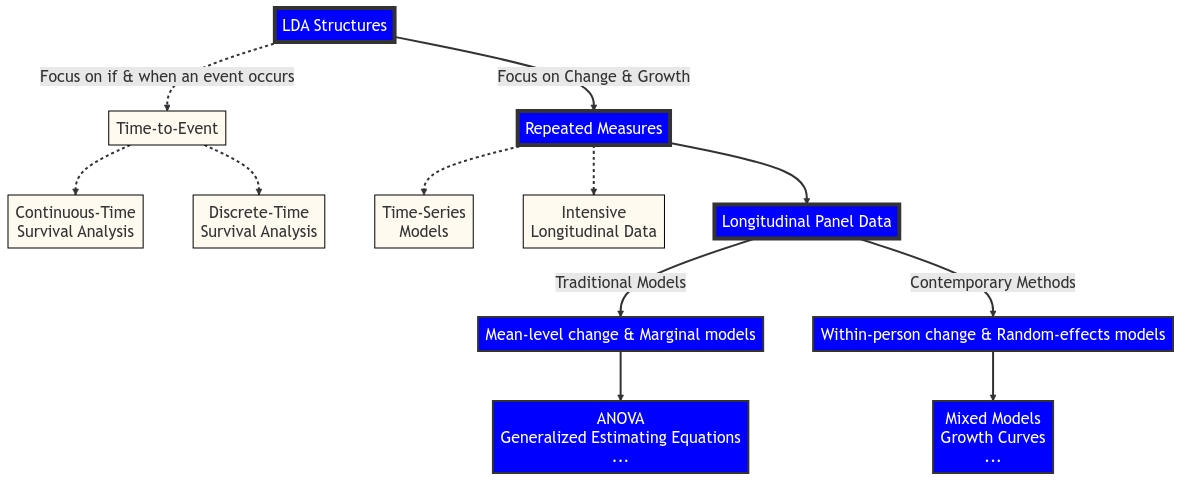
\includegraphics{./figures/LDAStructure2.png}}

}

\caption{Longitudinal Data Analysis Structural Diagram}

\end{figure}

When discussing longitudinal analysis, we are most often talking about
data collected on the same unit (e.g., individuals) across multiple
measurement occasions. However, repeated-measures analysis is not a
monolith, and it will serve us well to distinguish between a few of the
most common types. One such approach to repeated measures analysis is
the use of time-series models. These models generally consist of a long
sequence of repeated measurements (≧ 50-100 measurements) on a single
(or small number of) variable of interest. Time-series analysis is often
used to predict/forecast temporal trends and cyclic patterns and is
geared toward making inferences about prospective outcomes within a
population (with relatively with less focus on inferring
individual-level mechanisms and risk factors). A related type of
repeated measures analysis is Intensive Longitudinal Data (ILD). Similar
to time-series analysis, ILD models involve frequent measurements
(\textasciitilde{} 30-40 measurements) of the same individuals in a
relatively circumspect period of time (e.g., experience sampling to
obtain time series on many individuals). Although ILD models may include
slightly fewer measurement occasions than time-series data, ILD models
tend to have more subjects than time series models (\textasciitilde{}
50-100 subjects). This allows ILD models to examine short-term patterns
by incorporating a time series model that can sometimes fit parameter
estimates to each individual's data in order to model individual
difference outcomes. The final type of repeated measures analaysis that
we will discuss is the longitudinal panel model. These models follow a
group of individuals--- a panel (also referred to as a cohort) ---
across relatively fewer measurement occassions (\textasciitilde{} 5-15),
and are often interested in examining change across both,
within-individuals and between-individuals.

While other longitudinal designs have their own unique strengths and
applications, the longitudinal panel design is particularly well-suited
for investigating developmental processes in the context of the ABCD
Study. In the following sections, we will discuss various analytic
methods commonly used to analyze longitudinal panel data, including
growth models, mixed models, and a number of additional trajectory
models. These methods provide valuable insights into within- and
between-individual differences and are highly relevant for researchers
working with the ABCD Study dataset. By focusing on these methods, we
aim to equip readers with the knowledge necessary to conduct
longitudinal research and perform analyses using the rich, longitudinal,
and publicly available data from the ABCD Study.

\hypertarget{longitudinal-analysis}{%
\section{Longitudinal Analysis}\label{longitudinal-analysis}}

\label{sec:headings}

\hypertarget{types-of-longitudinal-panel-models}{%
\subsubsection{Types of longitudinal panel
models}\label{types-of-longitudinal-panel-models}}

With the large and continually expanding body of research on statistical
methods for longitudinal analyses, determining which longitudinal model
to implement can be challenging. The aim of this section is to help
researchers navigate these many options to identify the statistical
approach most appropriate to their unique research question. Notably,
there are a myriad of viable ways one can go about grouping various
types of longitudinal models for presentation.

Common examples include grouping by linearity {[}linear vs nonlinear
models; see \citep{collins2006}{]}, the number of measurement occasions
\citep[see][]{king2018}, and statistical equivalency {[}e.g., change
scores vs.~residualized change; see \citep{castro-schilo2018}{]}. The
organization we use below overlaps in a number of ways with these
examples, and in particular with \citep{bauer2019}. However, it is
important to note that in each case, the ordering that is chosen is
somewhat arbitrary and primarily intended to allow the reader to compare
and contrast various analytic approaches. In the following we describe
(briefly) and summarize the advantages/disadvantages of a series of
longitudinal models organized into the following groupings: Traditional
Models, Modern GLM Extensions, SEM, and Advanced SEM. We note that this
is not an exhaustive review of each of these methods, but for more
in-depth detail we do provide the reader relevant resources
\citep[e.g.,][]{curran2021}. As aptly summarized by \citep{bauer2019},
``there are many exceptions, alternatives, nuances, `what ifs', and `but
couldn't yous' that aren't addressed here.''

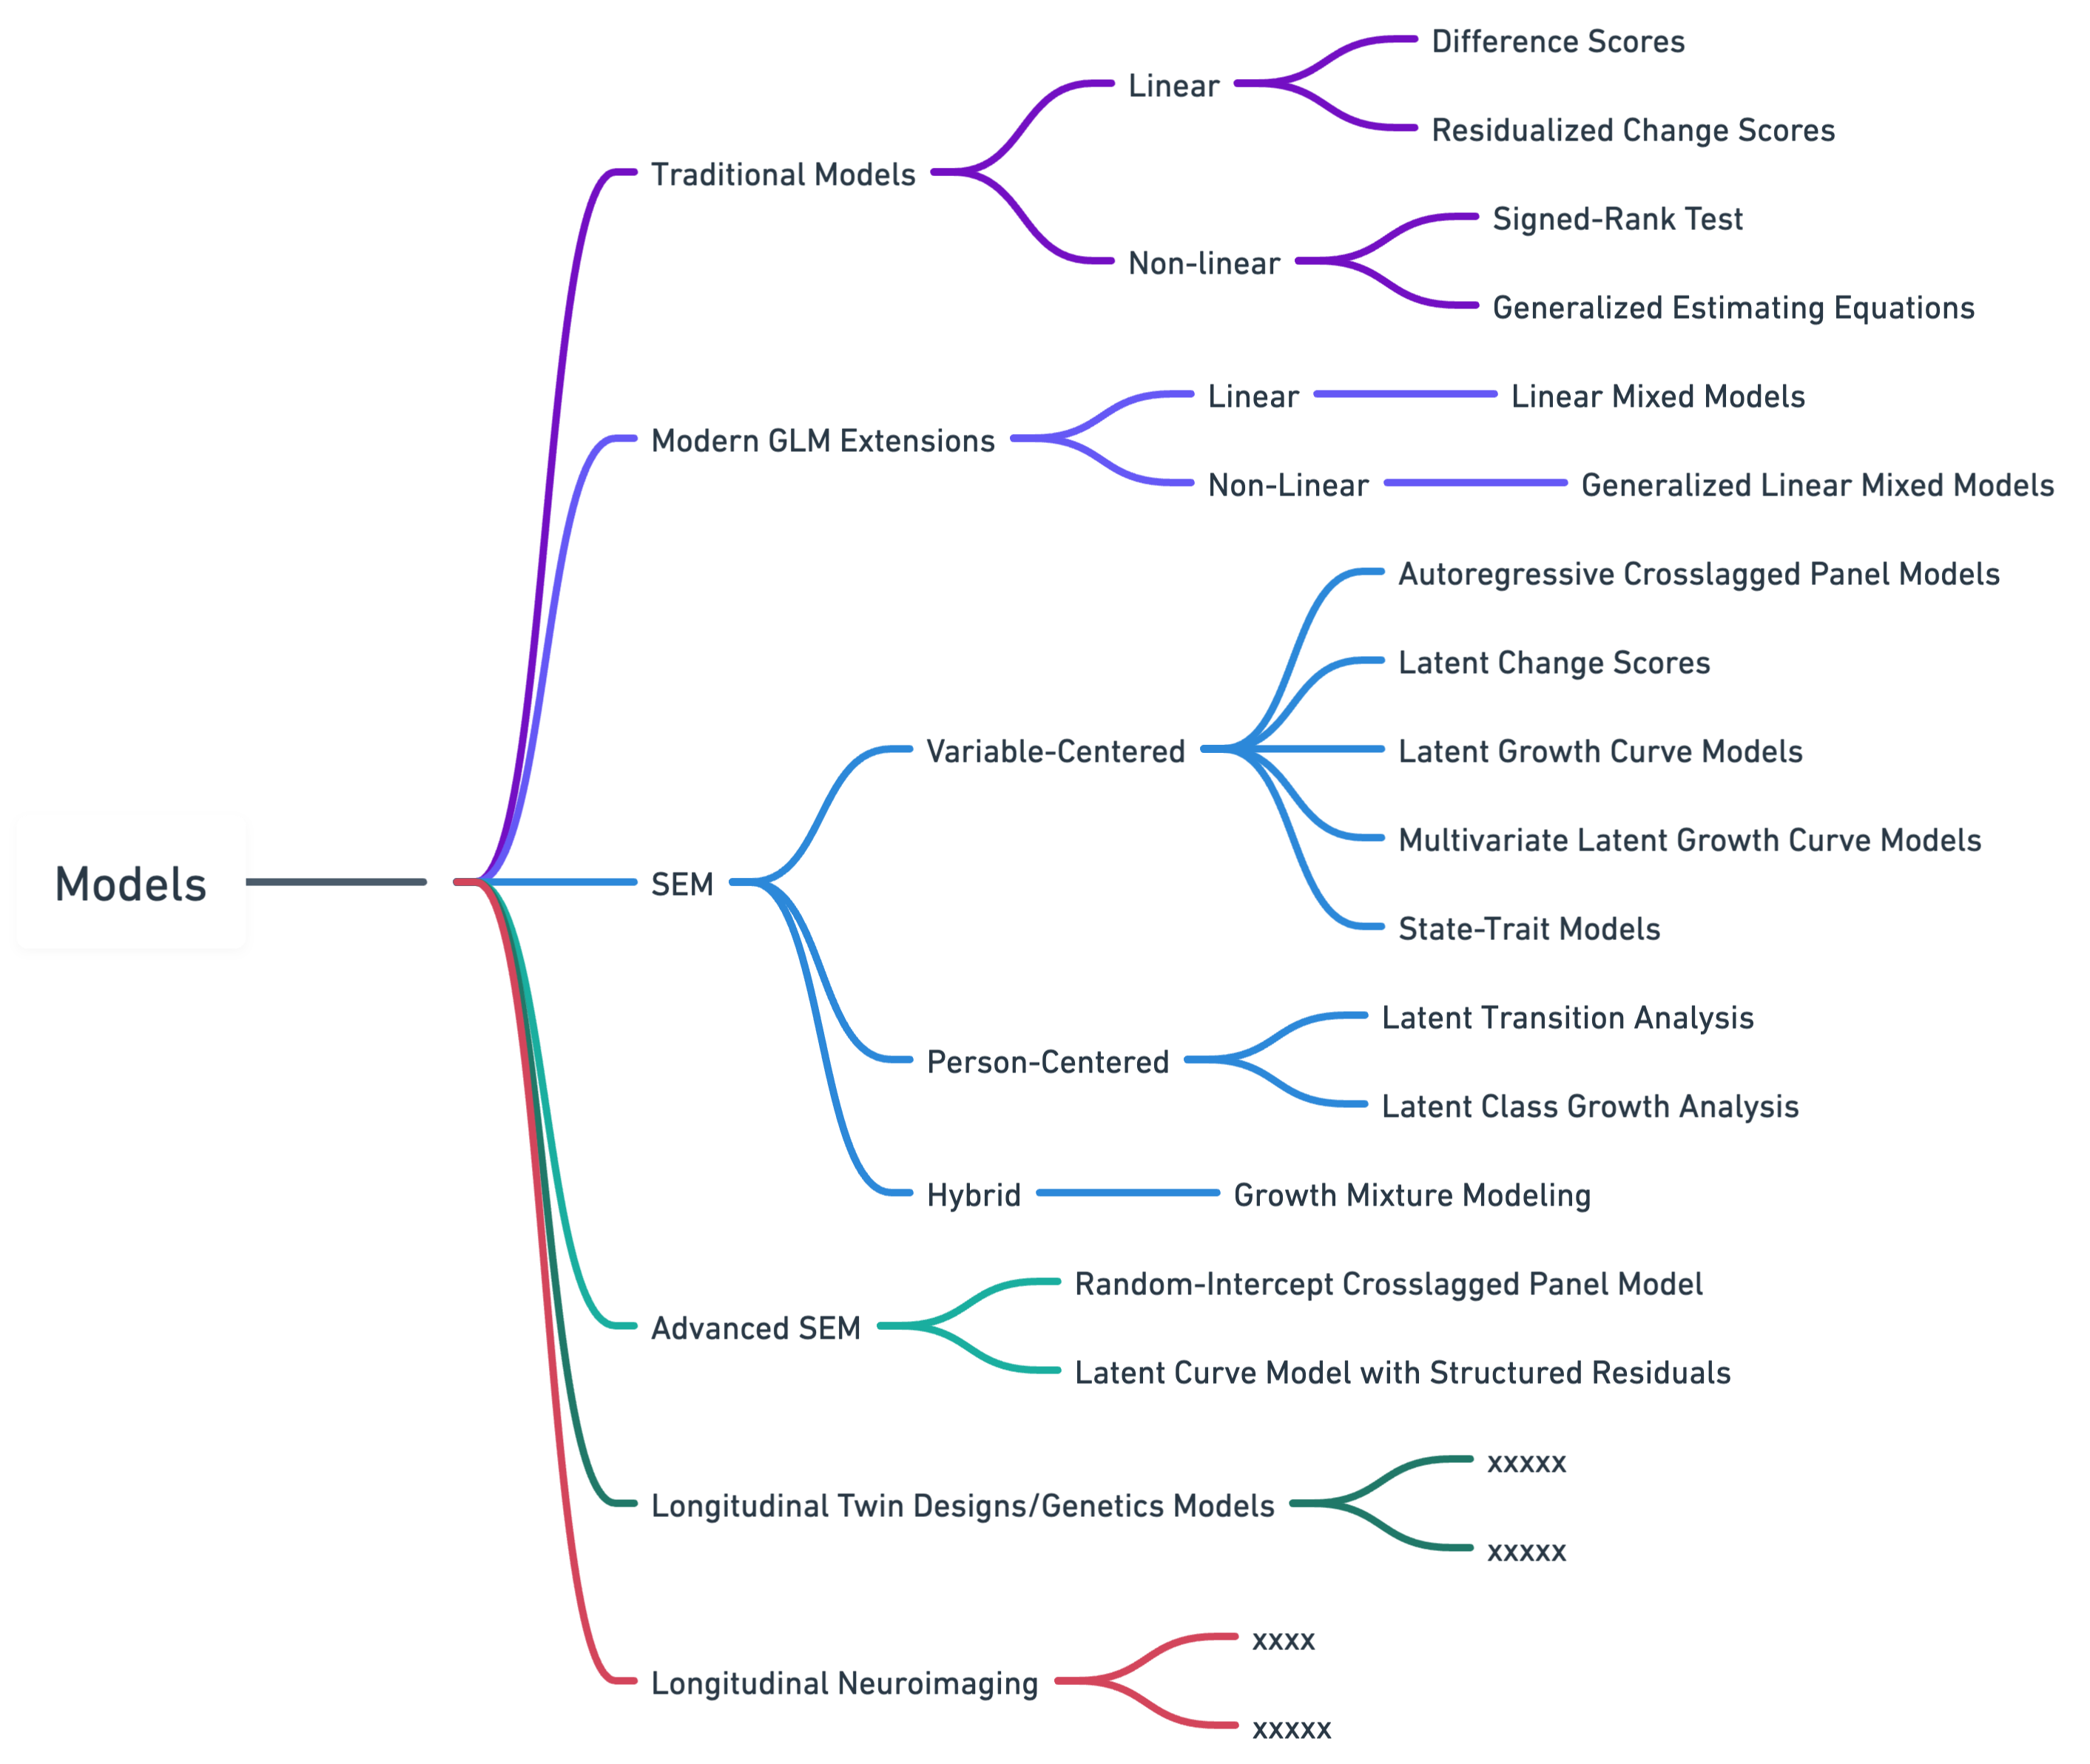
\includegraphics[width=3.125in,height=3.125in]{./figures/Mindmap1copy.png}

\hypertarget{traditional-models}{%
\paragraph{Traditional Models}\label{traditional-models}}

Traditional methods for longitudinal analysis primarily focus on
modeling mean-level change, and how these changes may differ across
groups or levels of some other variable. For example, is there a
difference in average math scores obtained across multiple assessments
between boys and girls? Longitudinal models that focus on mean-level
change are also referred to as marginal models and examples of specific
methods include repeated measures ANOVA (and MANOVA), ANCOVA, and
Generalized Estimating Equations (GEE). These methods are commonly used
when data is only available from 2 measurement occasions. For example,
computing a difference score (e.g., math scores at t2 - math scores at
t1) that can be used as an outcome in a subsequent GLM analysis (e.g.,
paired-samples t-test, repeated measures ANOVA) to test for differences
in patterns of change over time and between groups. Additionally, the
longitudinal signed-rank test, a nonparametric alternative to the paired
t-test, can be a useful tool for analyzing non-normal paired data.
Another common approach, often used in pre-/post-design studies, is to
use residualized change score analysis to assess the degree of change in
a variable, while controlling for its initial level. For example,
regressing post-treatment scores on pre-treatment scores and then using
the resulting residuals as a measure of change that is adjusted for
baseline scores (ignoring any prior group assignments/differences).
Similar to difference scores, the residualized change score is often
included in subsequent analyses, such as for evaluating intervention
effects in pre-test/post-test designs \citep{kisbu2013}.

Traditional longitudinal methods can still be useful in some contexts
(e.g., \textless{} 3 measurement occasions), but their practical utility
for answering questions about developmental processes is limited.
Perhaps most notably, these models do not allow for characterizing
patterns of within-person change. This is a particularly important
limitation since most psychological theories posit within-person
processes (i.e., what will happen within a given individual). As such,
traditional approaches often correspond poorly with most theoretical
models of change and a failure to disaggregate between-person and
within-person effects can result in consequential errors of inference
(e.g., ecological fallacy) \citep{curran2011}. Moreover, even
determining which of these procedures to use for comparing change over
two time points across groups can be surprisingly complicated. A
particularly vexing example is that of imbalanced baseline scores (i.e.,
when baseline scores are correlated with a covariate of interest), which
can produce different conclusions across methods \citep[see][for a
review]{littlefield2023}. Given these shortcomings, and the complexity
of the issues surrounding some of these methods, it is typically
recommended that researchers make use of more modern approaches for
analyzing longitudinal data (and preferably make use of data collected
across 3 or more time points).

\hypertarget{modern-glm-extensions}{%
\paragraph{Modern GLM Extensions}\label{modern-glm-extensions}}

Modern approaches to longitudinal data analysis have advanced beyond
traditional methods by offering greater flexibility and a more in-depth
understanding of within-person and between-person variability.
Generalized Estimating Equations (GEE), Linear Mixed Models (LMM),
Generalized Linear Mixed Models (GLMM), and Autoregressive Cross-Lagged
Panel Models (ARCL) are examples of such contemporary techniques. GEE,
an extension of Generalized Linear Models, combines the generalized
linear model for non-normal outcomes with repeated measures (marginal)
model and is suitable for analyzing correlated longitudinal data and
modeling population-averaged effects. LMMs, also known as multilevel or
hierarchical linear models, facilitate the simultaneous analysis of
within-person and between-person variability, making them ideal for
nested data structures or repeated measures. GLMMs further extend the
LMM framework to accommodate non-normal response variables, such as
binary, count, or ordinal data. Finally, ARCL models are used to
investigate reciprocal relationships between variables over time, as
they estimate both autoregressive and cross-lagged effects {[}although,
ARCL models are relatively less useful for teasing apart between-person
and within-person sources of variances; see \citep{curran2021}{]}.

The strengths of these modern methods lie in their ability to account
for individual differences, within-person change, and time-varying
predictors, thereby providing a more comprehensive understanding of
complex relationships in longitudinal data. Despite these advantages,
modern approaches may require more complex modeling assumptions and
higher computational demands compared to traditional methods.
Additionally, proper model specification and the interpretation of
results can be more challenging, especially in cases of high
multicollinearity or missing data. However, modern longitudinal analysis
methods have generally surpassed traditional methods in addressing a
wider range of research questions, accommodating diverse data
structures, and elucidating the intricate dynamics of developmental
processes.

\hypertarget{sem}{%
\paragraph{SEM}\label{sem}}

Structural equation modeling (SEM) approaches have gained prominence in
longitudinal data analysis due to their ability to estimate complex
relationships among observed and latent variables while accounting for
measurement error. SEM techniques can be categorized into
variable-centered, person-centered, and hybrid approaches, each with
unique strengths and limitations. The choice of method depends on the
research question, data structure, and underlying assumptions.

Variable-centered approaches, such as latent change scores, latent
growth curve models, multivariate (parallel process) latent growth curve
models, and latent state-trait models, focus on examining relationships
among variables and population-level patterns. These models offer a
powerful means to estimate individual change trajectories and the
relationships between growth parameters of different variables, while
also decomposing observed measurements into latent state and trait
components. However, these approaches may not adequately capture
distinct subgroups of individuals who share similar patterns of change
over time, which can be crucial for understanding heterogeneous
developmental processes.

Person-centered approaches, including latent transition analysis and
latent class growth analysis, address this limitation by identifying
subgroups of individuals who share similar patterns of change. These
models can reveal meaningful subpopulations and help researchers
understand the factors that contribute to differences in developmental
trajectories. Nevertheless, person-centered methods may overlook
important relationships among variables, which can be essential for
understanding the dynamics of change over time.

Hybrid approaches, such as growth mixture modeling, combine aspects of
both variable-centered and person-centered models, allowing for the
identification of latent subgroups while also modeling relationships
among growth parameters. This combination provides a more comprehensive
understanding of longitudinal data by capturing both within- and
between-person variability. However, hybrid models can be more complex,
necessitating careful model specification, selection, and
interpretation. Additionally, these methods may require larger sample
sizes to ensure the stability and accuracy of results.

In summary, SEM approaches offer powerful tools for longitudinal data
analysis, enabling researchers to investigate complex relationships,
individual differences, and change dynamics over time. The choice
between variable-centered, person-centered, and hybrid approaches
depends on the research objectives and the nature of the data. Despite
their limitations, these models have greatly advanced our understanding
of developmental processes and the factors that contribute to individual
differences in change trajectories.

\hypertarget{advanced-sem}{%
\paragraph{Advanced SEM}\label{advanced-sem}}

Advanced structural equation modeling (SEM) approaches, such as the
random-intercept cross-lagged panel model (RI-CLPM) and latent curve
models with structured residuals (LCM-SR), have emerged to address more
complex research questions and data structures in longitudinal analysis.
These advanced models extend traditional SEM techniques, enabling
researchers to disentangle within-person and between-person effects, as
well as capture additional time-specific dependencies and associations
that may not be accounted for by the latent growth factors.

The RI-CLPM enhances the traditional cross-lagged panel model by
incorporating random intercepts, which allow for the separation of
stable individual differences from the dynamic within-person
associations among variables over time. Within-person variance in these
models are captured by a series of latent variables that reflect time
specific variance (i.e., the residual variance from the random
intercept). These time-specific variables are referred to as structured
residuals. Distinguishing between-person variance subsumed by the random
intercept from the structured residuals is particularly valuable for
understanding the time-specific effects of one variable on another,
while accounting for the influence of individual differences. However,
RI-CLPM may require larger sample sizes to ensure stability and accuracy
of the estimates and can be computationally demanding.

LCM-SR, on the other hand, extends the RI-CLPM by including additional
growth factors, such as a random linear slope. That is, the LCM-SR is a
hybrid between a latent growth model and CLPM. This approach allows for
a more comprehensive understanding of within-person change dynamics and
factors influencing change over time. By including structured residuals,
LCM-SR can capture additional time-specific relationships that are not
explained by the latent growth factors. However, even more so than the
RI-CLPM, LCM-SR comes with increased model complexity and requires
careful specification and interpretation.

In conclusion, advanced SEM approaches for longitudinal data analysis
provide valuable tools for addressing complex research questions and
data structures. While they offer more nuanced insights into
within-person change dynamics and the influence of individual
differences, these models also come with certain limitations, such as
the necessity of multiple assessments (e.g., four or more for LCM-SR),
increased complexity, computational demands, and the need for careful
model specification and interpretation. As with any statistical method,
researchers should carefully consider their research objectives, data
characteristics, and the assumptions of each model when selecting the
most appropriate advanced SEM approach for longitudinal analysis.

\begin{figure}

{\centering 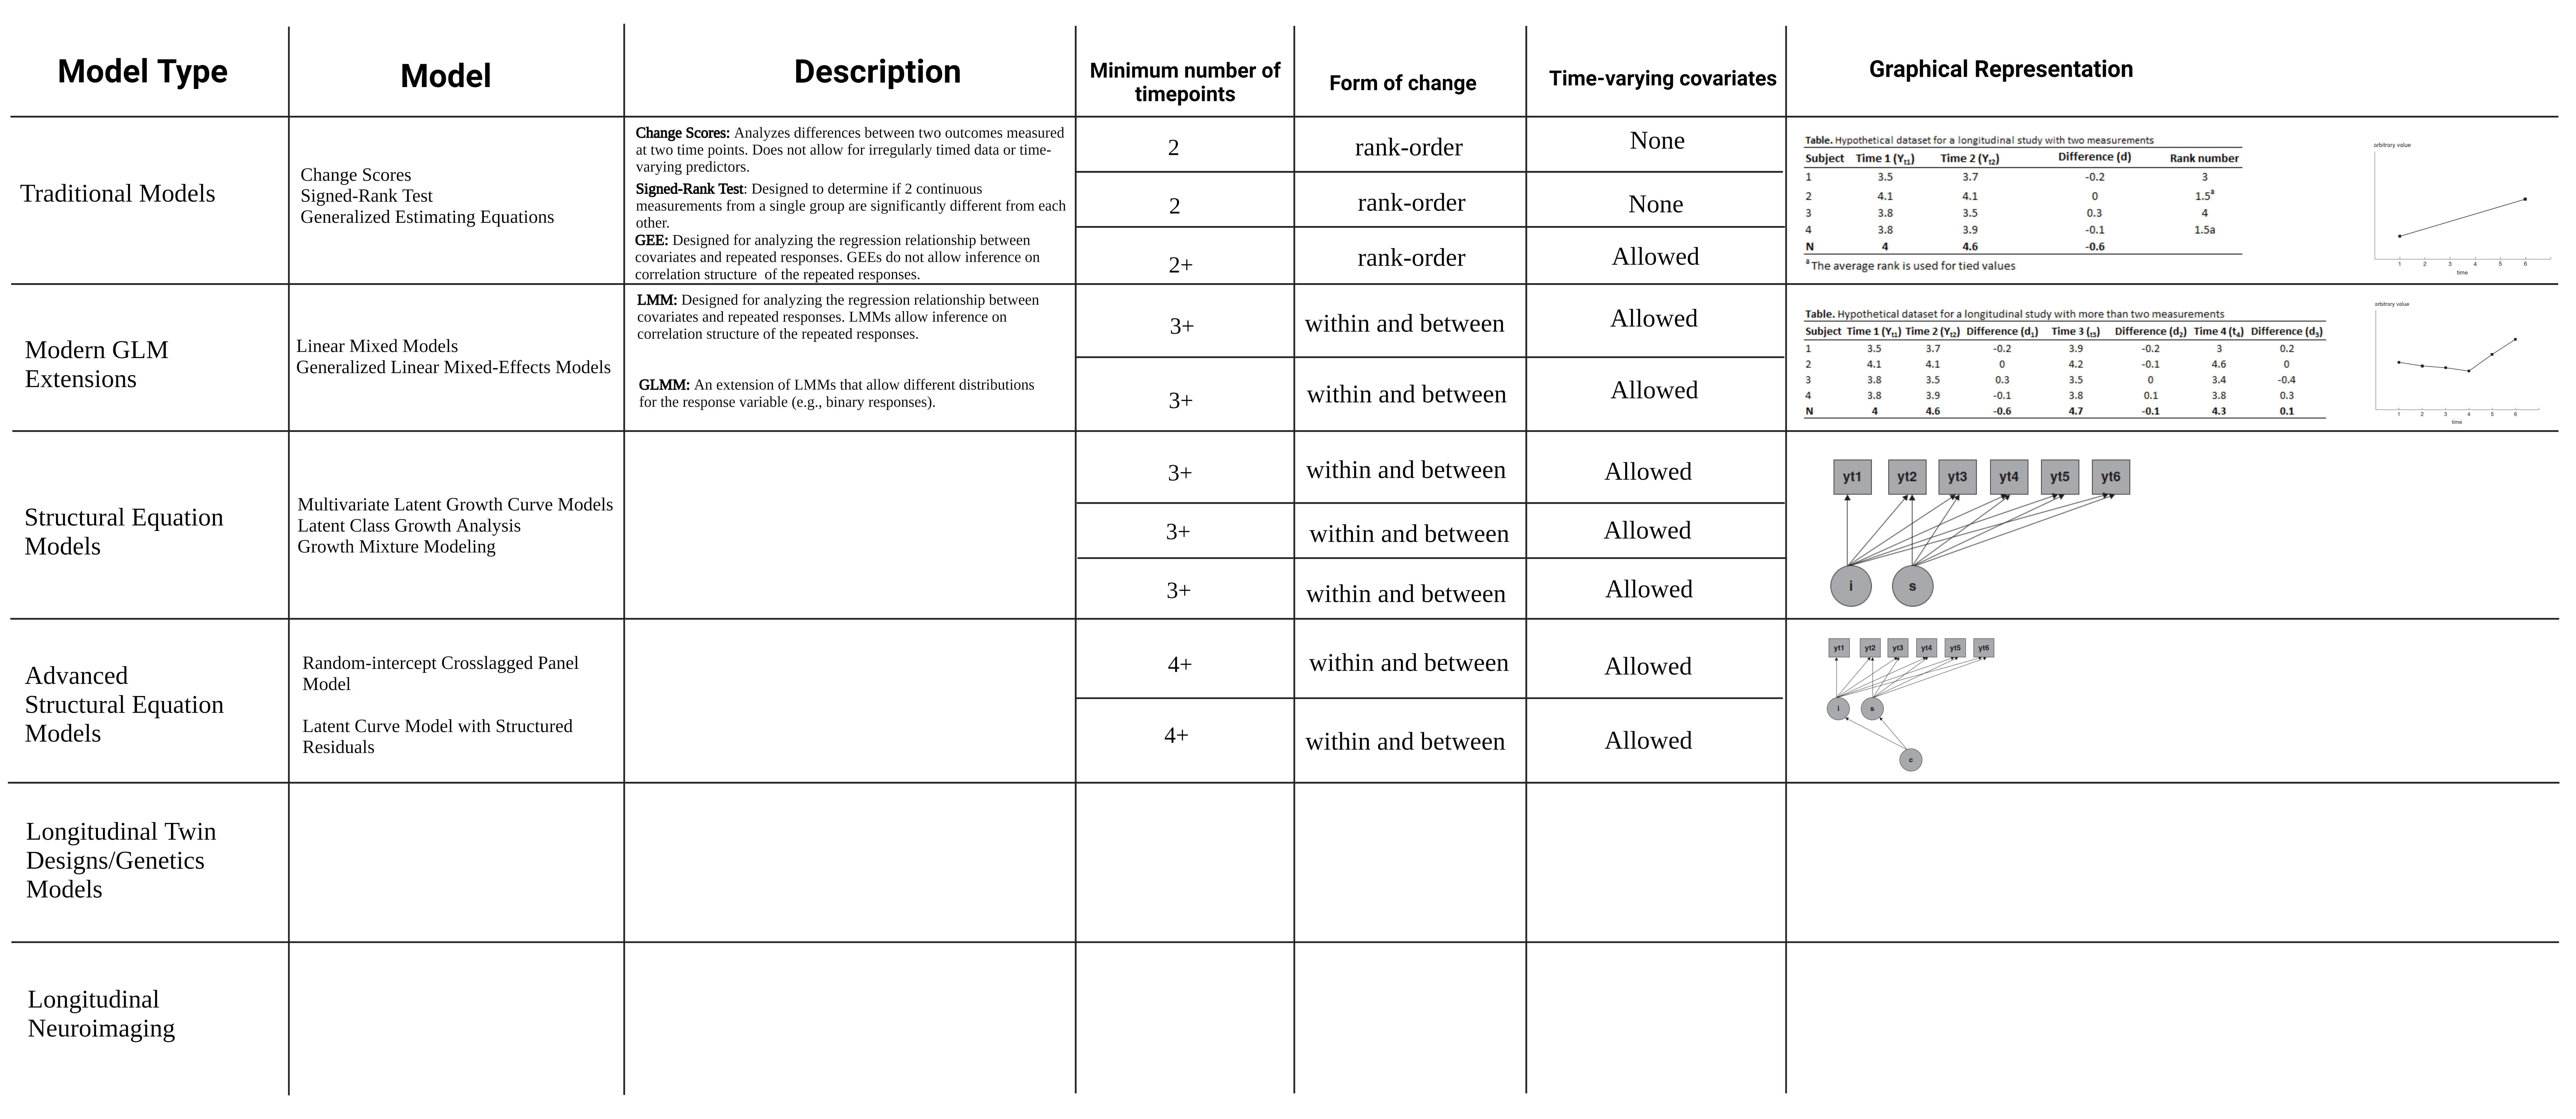
\includegraphics{./figures/Tabletemp.png}

}

\caption{LDA Table}

\end{figure}

\hypertarget{discussion}{%
\section{Discussion}\label{discussion}}

\label{sec:headings}

As we enter the era of large-scale longitudinal investigations, it is
essential to critically examine the various analytical methods that can
be employed to glean insights from these rich datasets. The complex
nature of longitudinal data demands sophisticated and well-suited
methodologies to accurately address research questions and minimize
biases. This paper aimed to provide a comprehensive review of diverse
longitudinal analysis techniques, with a particular emphasis on their
application to extensive longitudinal studies such as the ABCD Study.
Beyond contributing to the ever-growing body of knowledge on
longitudinal data analysis, we hope this manuscript also serves as a
valuable resource for researchers seeking to optimize the use of
large-scale longitudinal investigations in advancing our understanding
of human development and behavior. In this discussion, we will focus on
the key findings and recommendations of our review and discuss potential
innovations that can further enhance the utility of these methods.

We began by addressing fundamental concepts and considerations in
longitudinal research that are essential for generating accurate and
meaningful insights into developmental processes. Concepts such as
vulnerable periods, developmental disturbances and snares, or cascade
and experience effects (among many others), are instrumental in shaping
the design, analysis, and interpretation of longitudinal studies. For
example, understanding and accounting for vulnerable periods and
developmental disturbances in research designs allows researchers to
investigate the timing and magnitude of the impact of specific factors
on development, while snares and cascade effects demonstrate the
importance of considering the interconnectedness of developmental
processes. Together, these concepts provide a framework for
understanding the mechanisms underlying the course of development, while
also accounting for the complex interplay between individual development
and the influence of environmental factors. By considering the intricate
relationships among these factors, researchers can better identify the
critical time periods, situations, and contexts that contribute to
individual differences in developmental outcomes. This awareness enables
more precise inferences regarding the causal relationships between
exposures and outcomes, ultimately leading to more robust and meaningful
findings that can help facilitate the translation of research findings
into practical applications in clinical and public health settings.

We also discussed some of the opportunities, challenges, and pitfalls
that arise when working with longitudinal data. Key issues include
selecting appropriate methods to account for the intricacies of
longitudinal data, addressing missing data in a way that minimizes
biases, and determining suitable longitudinal data structures that align
with research questions and context. To address these challenges,
researchers should carefully consider issues such as study design,
selection of methods that account for both within- and between-person
sources of variance, and employing modern techniques, (e.g., FIML,
multiple imputation) for handling missing data. By adhering to best
practices in longitudinal research and remaining vigilant of potential
pitfalls, researchers can effectively harness the power of longitudinal
data to maximize the potential of their investigations and gain valuable
insights into complex developmental processes, individual differences,
and the underlying mechanisms that drive change over time.

The final section, along with associated code and additional resources
made available as online supplements (), aims to serve as a resource for
researchers seeking to understand and implement various longitudinal
panel models. By providing an overview of different approaches, their
strengths and limitations, and key considerations for their use, we hope
to facilitate the selection of appropriate models tailored to specific
research questions and data structures. It is essential for researchers
to consider their research objectives, the characteristics of their
data, and the assumptions underlying each model when choosing the most
suitable approach for longitudinal analysis. We encourage researchers to
consult the cited literature and online supplements for further guidance
in selecting and implementing longitudinal models when using the ABCD
Study dataset. As the field continues to advance, we anticipate the
emergence of new methods and refinements to existing approaches, further
expanding the toolkit available to researchers for the analysis of
longitudinal data. By staying informed about developments in this area
and critically evaluating the appropriateness of different models for
their research questions, researchers can ensure that their longitudinal
analyses are both rigorous and informative. Notably, in this vast and
continually evolving field, with numerous models and approaches
available to address a wide range of research questions, no single model
is universally applicable or without limitations. The diversity of
methods ensures that researchers can find an appropriate tool for their
specific needs. By familiarizing themselves with the various types of
longitudinal models, researchers can more effectively navigate the
complexities of longitudinal data and contribute valuable insights into
the developmental processes and individual differences that shape human
experience.

\newpage{}


\renewcommand\refname{Part V: References}
  \bibliography{../references.bib}


\end{document}
